% !TeX program = xelatex
% Editable narrative; numeric blocks/figures are regenerated from frozen evidence.
\documentclass[10pt,a4paper,twocolumn]{article}
\usepackage{fontspec}
\IfFontExistsTF{Times New Roman}{\setmainfont{Times New Roman}}{\setmainfont{Libertinus Serif}}
\IfFontExistsTF{Arial}{\setsansfont{Arial}}{\setsansfont{DejaVu Sans}}
\IfFontExistsTF{Consolas}{\setmonofont{Consolas}}{\setmonofont{Latin Modern Mono}}
\usepackage[russian]{babel}
\usepackage[margin=18mm,top=19mm,bottom=19mm,footskip=9mm]{geometry}
\usepackage{amsmath,amssymb,booktabs,microtype,graphicx,xcolor,titlesec,fancyhdr}
\usepackage[font=small,labelfont={bf,sf},labelsep=period]{caption}
\usepackage[colorlinks=true,linkcolor=black,urlcolor=teal,citecolor=teal]{hyperref}
\definecolor{ink}{HTML}{243747}\definecolor{teal}{HTML}{167889}\definecolor{muted}{HTML}{657785}
\setlength{\columnsep}{7mm}\setlength{\parindent}{.8em}\setlength{\parskip}{1.5pt}
\setlength{\headheight}{14pt}\setlength{\textfloatsep}{9pt}\setlength{\dbltextfloatsep}{10pt}
\emergencystretch=2em\clubpenalty=10000\widowpenalty=10000\displaywidowpenalty=10000
\titleformat{\section}{\sffamily\bfseries\fontsize{11}{13}\selectfont\color{ink}}{\thesection}{.6em}{}
\titlespacing*{\section}{0pt}{9pt}{4pt}
\titleformat{\subsection}{\sffamily\bfseries\fontsize{9.5}{11.5}\selectfont}{\thesubsection}{.5em}{}
\titlespacing*{\subsection}{0pt}{6pt}{3pt}
\pagestyle{fancy}\fancyhf{}
\fancyhead[L]{\sffamily\fontsize{7}{8}\selectfont\color{muted}REWARD MODEL И ВЫБОР ДЕЙСТВИЯ}
\fancyhead[R]{\sffamily\fontsize{7}{8}\selectfont\color{muted}YAMBDA / GPT-2 / ВТОРОЙ ЦИКЛ}
\fancyfoot[C]{\sffamily\small\thepage}\renewcommand{\headrulewidth}{.25pt}
\setcounter{dbltopnumber}{1}
\raggedbottom
\newcommand{\EvalUsers}{637}
\newcommand{\EvalQueries}{6393}
\newcommand{\SftNdcg}{0.010095}
\newcommand{\CeNdcg}{0.012977}
\newcommand{\GatedNdcg}{0.012880}
\newcommand{\GainPercent}{28.5}
\newcommand{\RmMse}{0.059784}
\newcommand{\OldRmMse}{0.184392}
\newcommand{\PrimaryDelta}{-0.000096}
\newcommand{\PrimaryLo}{-0.000162}
\newcommand{\PrimaryHi}{-0.000037}
\newcommand{\CopyDelta}{+0.002882}
\newcommand{\CopyLo}{+0.001290}
\newcommand{\CopyHi}{+0.004613}

\begin{document}
\twocolumn[{
\begin{center}
{\sffamily\bfseries\fontsize{19}{22}\selectfont\color{ink}Точнее предсказывать отклик\\недостаточно для полезного RL\par}
\vspace{5pt}
{\sffamily\fontsize{10}{12}\selectfont Copy-адаптер GPT-2, сильная reward model и проверка согласия моделей\par}
\vspace{5pt}
{\sffamily\fontsize{8}{10}\selectfont\color{muted}Воспроизводимое исследование на Yambda 50M / Октябрь 2026\par}
\end{center}
\vspace{3pt}
\noindent\textbf{Аннотация.} В первом цикле RL-донастройки GPT-2 модель отклика
едва превосходила константу, а почти половина целей находилась вне словаря.
Мы добавили обучаемый механизм копирования из реальной истории и RM с
историческими откликами. На новой заранее выделенной когорте из \EvalUsers{}
активных пользователей улучшенный supervised baseline повысил NDCG@10
с \SftNdcg{} до \CeNdcg{} (+\GainPercent\%). MSE новой RM снизилась с
\OldRmMse{} у прежней сети до \RmMse{}. Однако главный вариант joint CE+reward,
допускающий награду при согласии трёх RM, уступил продолжению CE:
$\Delta=\PrimaryDelta$, 95\% user-cluster CI $[\PrimaryLo;\PrimaryHi]$.
Показываем, что высокая точность отклика во многом объясняется состоянием
пользователя, а ошибки ансамбля сильно коррелируют. Это ограничивает
полезность общей MSE и согласия RM как критериев допуска reward-градиента.
\vspace{9pt}
}]

\section{От слабой RM к проверяемому контролю}

Предсказание следующего трека и оптимизация ожидаемого отклика решают разные
задачи. Для второго шага нужна модель $r(h,a)$, но низкая ошибка на logged
actions ещё не означает правильного порядка ненаблюдавшихся кандидатов.
Пользователь, который обычно дослушивает музыку, предсказуем независимо от
того, какой из нескольких треков ему рекомендовать.

В первом цикле мы обучили GPT-2 и выполнили REINFORCE с пятью наградами.
Выбранные варианты не подтвердили прирост NDCG; ансамблевая RM имела
MSE 0,180 против 0,181 у константы. Пятишаговая генерация повышала прогноз
RM, когда собственные рекомендации добавлялись в контекст без наблюдения
отклика. Штраф за этот сдвиг не помог. Полный журнал первого цикла сохранён
отдельно; его открытый test не используется для нового подбора.

Здесь проверяем более узкий вопрос: поможет ли reward после усиления RM
и supervised baseline? Наша модификация разрешает reward-обновление, когда
три RM согласны о направлении предпочтения между генерацией GPT-2 и copy.
Согласие не трактуется как доверительная граница. Основной контраст
заранее задан: gated joint против дополнительного CE той же модели.

\begin{figure*}[t]
\centering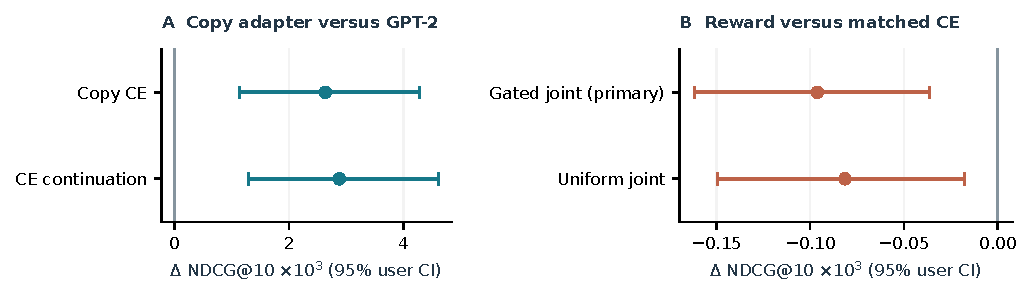
\includegraphics[width=.97\textwidth]{figures/effects.pdf}
\caption{Прирост copy и эффект reward разделены. A: улучшение supervised baseline
относительно GPT-2. B: reward уступает matched CE; gated --- основной контраст.
Оси имеют разные масштабы. Интервалы:3000 парных resamples пользователей,
метрики предварительно усреднены по трём model seeds. Контрольные CI описательные.}
\label{fig:effects}
\end{figure*}

\section{Данные, время и поддержка действий}

Использован pinned Yambda flat/50m, revision
\texttt{dd6f3a19eef5\ldots}. Из 9238 исходных UID исключены когорты v3/v4
и все 1200 UID первого Task 2. Равномерно выбраны 1000 других UID, seed 161803;
сохранены все 5\,130\,518 строк шести исходных колонок.
Новая когорта не участвует в обучении. Это перенос на другие UID
\emph{того же периода}, не независимая будущая неделя.

Обучение использует прежние 1200 UID до day 270. Development: прежние 800 UID,
days 280--286. Новый test: days 293--298. Query --- первые до 4 неорганических
событий с уникальным timestamp за user-day. Входы содержат только события
строго раньше запроса; одновременные события не упорядочиваются причинно.
Оценены \EvalQueries{} запросов \EvalUsers{} пользователей.

Общий train-каталог содержит 270\,376 треков. GPT-2 имеет 16\,384 head-токена;
copy получает последние 64 исходных item IDs, включая tail, если item
наблюдался в train-каталоге. Полный каталог покрывает 80,7\% test-целей,
head --- 48,6\%, достижимая поддержка head+copy --- 49,9\%.
Copy исправляет только часть OOV: tail вне последней истории остаётся
недостижимым. Все пропущенные цели дают 0, positives не добавляются.

\section{Модели и цель оптимизации}

\subsection{Замороженный decoder и copy-адаптер}
GPT-2 первого цикла:3 pre-LN causal blocks, width 128,4 heads, context 64,
2,70млн параметров, обучение с нуля на ID. Checkpoint и три seeds17/42/73
сохраняются. Дополнительных SFT fits в этом цикле нет.

Для frozen распределения $p_0$ и последних 64 событий задаём
\begin{equation}
p_\theta(a\mid h)=(1-g_\theta(h))p_0(a\mid h)
+g_\theta(h)\!\sum_{j:h_j=a}c_\theta(j\mid h).
\end{equation}
Gate --- sigmoid от 13 признаков реальной истории и bias. Copy softmax
имеет обучаемый recency decay и вес прошлого completion. Всего 16
обучаемых параметров. Масса повторных позиций суммируется; неизвестные
каталогу items не копируются. Это облегчённая адаптация политики,
а не дообучение всех параметров трансформера.

Механизмы copy и repeat--explore известны по Pointer Sentinel~\cite{pointer}
и RepeatNet~\cite{repeat}. Проверяемая идея этой работы --- admission
критерий для reward, а не новый механизм копирования.

\subsection{Reward model с историческими откликами}
Три CatBoostRegressor предсказывают
$y=\operatorname{clip}(\texttt{played\_ratio\_pct}/100,0,1)$.
Входы:13 признаков состояния (прошлые completion, пропуски, длина истории,
временной gap и др.) и 7 признаков кандидата (счётчики, сглаженный completion,
длительность, повторы и давность). Outcomes текущего события исключены.

Статические item aggregates зафиксированы до day 200. RM train --- days 200--259,
calibration --- 260--269; максимум 150/30 примеров на пользователя, исходные
истории не урезаются. Глубины 4/6, до 400 деревьев; выбор только по calibration
MSE. Выбрана глубина 6. Раннее прекращение отдельно для каждого seed.
Два дополнительных диагностических контроля используют только состояние
или только item statistics. Исторический отклик считается доступным по
timestamp лога; реальные задержки доставки неизвестны.

\begin{figure*}[t]
\centering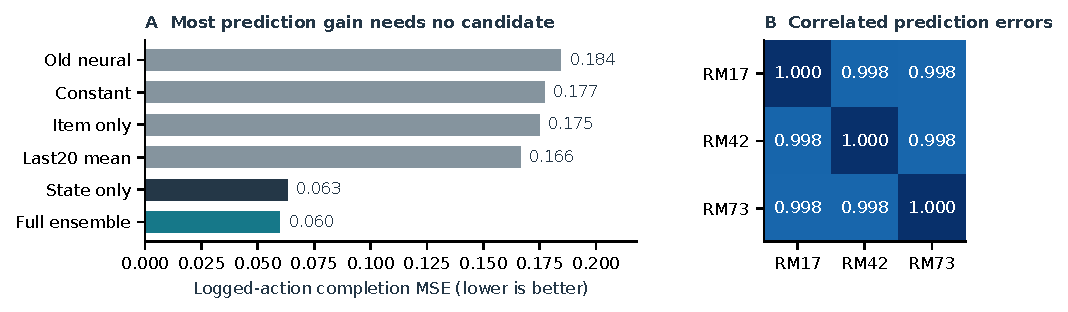
\includegraphics[width=.97\textwidth]{figures/reward.pdf}
\caption{Новая RM точнее, но большая часть прогнозируемости связана с состоянием.
State-only --- одна модель; full --- ансамбль трёх, поэтому это не идеально
уравненная абляция ансамблей. Справа: корреляция ошибок трёх полных RM на
logged actions. Их согласие не является независимым подтверждением.}
\label{fig:rm}
\end{figure*}

\subsection{CE, reward и критерий допуска}
CE-адаптер обучается до 1200 updates, batch 256, Adam lr 0,01; checkpoint
выбирается по development NDCG seed 17. Остальные seeds наследуют 1200.
Используется до 40 случайных contexts/user из days 240--269.
Затем все методы получают 300 updates с lr 0,003:
\begin{equation}
\mathcal L=\mathcal L_{CE}+0{,}1D_{KL}(q_\theta\Vert q_{CE})
-\lambda I(h)\widehat{\mathbb E}_{p_\theta}[r].
\end{equation}
Здесь $q$ --- совместное распределение branch и copy-position; его KL
ограничивает сверху KL marginal item-политики. Продолжение CE имеет
$\lambda=0$; reward-only убирает CE, сохраняя KL; uniform joint имеет $I=1$.
У gated $I=1$, если три RM согласны о знаке
$\mathbb E_c[r]-\mathbb E_{p_0}[r]$. Gate не читает logged target.

Ожидание по copy считается точно, по frozen GPT-2 --- по 8 MC samples/context.
Для такой смеси градиент ожидаемой награды доступен напрямую; REINFORCE
не требуется для этого конечного ожидания. Это H1 contextual-bandit RL
адаптера, не новый full-decoder H5 алгоритм. Сетка $\lambda\in\{0{,}1;0{,}5;2;8\}$,
все trials сохранены. Выбор --- максимальный development NDCG среди
настроек с proxy не ниже CE. Выбраны 0,1 для reward-only и 2 для joint/gated.
Подход AdaGRPO~\cite{ada} также сочетает NLL и селективный RL, но использует
ранги target/distractors; наш target-free критерий его не воспроизводит.



\section{Внешняя проверка}

\begin{table}[h]
\centering\small\setlength{\tabcolsep}{3pt}
\caption{Один test, общий каталог. Proxy --- прогноз completion top1,
не наблюдённая награда новой рекомендации.}
\begin{tabular}{lrrr}\toprule
Метод & NDCG@10 & Recall@10 & Proxy\\\midrule
Popularity & 0.003370 & 0.007510 & 0.6481 \\
Repeat / head & 0.008787 & 0.014725 & 0.6123 \\
Repeat / full & 0.011983 & 0.020471 & 0.6076 \\
GPT-2 & 0.010095 & 0.020913 & 0.6217 \\
Copy 50/50 & 0.011837 & 0.020592 & 0.6109 \\
Copy CE & 0.012731 & 0.025023 & 0.6187 \\
CE continuation & 0.012977 & 0.025332 & 0.6184 \\
Reward only & 0.012718 & 0.025030 & 0.6187 \\
Joint & 0.012895 & 0.025307 & 0.6186 \\
Gated joint & 0.012880 & 0.025267 & 0.6186 \\
\bottomrule\end{tabular}

\label{tab:ranking}
\end{table}

\textbf{Поддержка истории улучшила baseline.} Copy CE получил 0,012731
против \SftNdcg{} у GPT-2. После дополнительного CE --- \CeNdcg{},
+\GainPercent\%, абсолютная разность \CopyDelta{},
CI $[\CopyLo;\CopyHi]$ (рис.\ref{fig:effects}). Fixed copy50/50 слабее
обучаемой смеси. Превосходство над repeat не установлено: CE$-$repeat
0,000994, CI $[-0,001616;0,003283]$.

\textbf{Главный RL-контраст отрицателен.} Gated joint получил \GatedNdcg{}:
$\Delta=\PrimaryDelta$, CI $[\PrimaryLo;\PrimaryHi]$.
Это около$-0,74\%$ относительно CE. Uniform joint имеет сходное небольшое
снижение: $-0,000081$, CI $[-0,000150;-0,000018]$.
У gated proxy top1 вырос с 0,618404 до 0,618582, доля повторов снизилась
с 72,0\% до 71,6\%, средняя длительность --- с 189,2 до 189,1с.
На development gate пропускает 88,5\% contexts и потому мало отличается
от uniform joint. Первичный вывод относится к этому заранее заданному
критерию и бюджету, не ко всем вариантам RL.



\section{Что предсказывает сильная RM}

Новая RM имеет MSE\RmMse{} против \OldRmMse{} у прежней neural RM
и 0,176966 у константы той же train-популяции. Снижение относительно константы
66,2\%; event-weighted CI разности с user-cluster bootstrap
$[-0,124936;-0,109805]$. Сравнение RM включает добавление новой информации,
а не только замену архитектуры.

State-only без признаков кандидата имеет MSE 0,063096
(рис.\ref{fig:rm}). Одна эта модель достигает примерно 97\% сокращения MSE
полного ансамбля относительно константы. Full лучше неё:
CI разности $[-0,004046;-0,002591]$, но бюджет ансамбля различается.
Одна full RM seed 17 имеет MSE 0,059975; преимущество не объясняется только
усреднением. При этом корреляции ошибок полных RM около 0,998.

Эти наблюдения показывают ограничение критерия: хорошие прогнозы активности
пользователя дают низкую общую MSE, но сами по себе не создают полезного
преимущества одного действия над другим. Согласие похожих моделей также
не устраняет их общие ошибки. Это согласуется с reward overoptimization
и ограничениями ансамблей~\cite{overopt,ensemble}, хотя не устанавливает
единственную причину измеренного снижения NDCG.

Popularity имеет ещё более высокую proxy 0,648050 при NDCG0,003370.
Значит, «выше reward» в этой модели не совпадает с «точнее next item»
. Нет вероятностей показов и контрфактуальных
откликов: эти значения не являются IPS/DR оценкой или causal policy value.



\section{Воспроизводимость и границы вывода}

Полный SHA исходника и канонических значений всех шести колонок подтверждает
сохранение 5\,130\,518 строк новой когорты. Проверены отсутствие пересечений UID
и 62 замены будущего без изменения входов. Freeze связывает протокол, код,
выбранные рецепты и веса;24 массива прогнозов запечатаны до materialization
labels. CPU verifier пересчитывает ranking, RM errors, bootstrap и coverage
без исходного Yambda или GPU. Подмена чисел при обновлённом checksum также
отвергается replay-проверкой; это проверено отдельным тестом.

Описательный аудит длительности выполнен после test: используется медиана
из train до day 270. В frozen кэше RM значения до day 200 отсутствовали для
части треков и заменялись нулём; такой кэш занижал среднюю длительность.
Модели и первичные метрики не менялись.

В дополнительном цикле 24 fits адаптера и 6 RM fits, включая две диагностические
абляции. Записанные 30,5с адаптеров,27,2с кэшей и 6,3с основного RM поиска ---
времена отдельных этапов на RTX4070TiSUPER/i7-14700KF, не полная стоимость
исследования. Обучение прежнего GPT-2, подготовка, абляции, неудачные попытки
и ручная работа в эти времена не входят.

До labels исправлены выделение списка всего каталога для fallback и host
commit сбои. Первые freeze/код сохранены;22 уже вычисленных forecasts
остались побайтно идентичными. Никакие настройки по новому test не выбирались.

Границы результата существенны: один сервис и период, новая user-когорта,
637 активных UID, неполная поддержка действий и неизвестные задержки outcomes.
Адаптация имеет 16 параметров и H1; результат не переносится автоматически
на full-decoder H5 RL. Пятишаговая генерация первого цикла остаётся отдельным
аудитом вымышленной истории. Retention, удовлетворённость и настоящая
реакция на интервенцию требуют иных данных или online-проверки.

\textbf{Вывод.} Усиление supervised policy и RM дало воспроизводимый
измеримый результат. Дополнительный reward-сигнал в выбранной схеме
немного ухудшил релевантность. Проверять нужно не только точность RM
в среднем, но и её способность различать действия и независимость
ошибок моделей, на согласии которых строится admission.

\vspace{3pt}
\noindent\textbf{Код и данные результата.}\par
{\footnotesize\raggedright\noindent
\nolinkurl{reports/task2b/REPORT.md}; полный поиск --- \texttt{RESULTS.md}.\\
Протокол: \nolinkurl{docs/TASK2B_PROTOCOL.md}.\\
Проверка: \texttt{uv run --locked python}\\
\nolinkurl{scripts/verify_task2b.py}.\par}
\noindent Предыдущая статья и эксперименты сохранены отдельно.

\begin{thebibliography}{9}\small\setlength{\itemsep}{1pt}
\bibitem{pointer} Merity et al. Pointer Sentinel Mixture Models. ICLR 2017.
\href{https://arxiv.org/abs/1609.07843}{arXiv:1609.07843}.
\bibitem{repeat} Ren et al. RepeatNet: A Repeat Aware Neural Recommendation
Machine for Session-based Recommendation. AAAI 2019.
\href{https://arxiv.org/abs/1812.02646}{arXiv:1812.02646}.
\bibitem{ada} Xu et al. Adaptive Loss Balancing for Noise-Robust GRPO in
Generative Recommendation. Препринт 2026.
\href{https://arxiv.org/abs/2606.08480}{arXiv:2606.08480}.
\bibitem{overopt} Gao, Schulman, Hilton. Scaling Laws for Reward Model
Overoptimization. 2022. \href{https://arxiv.org/abs/2210.10760}{arXiv:2210.10760}.
\bibitem{ensemble} Coste et al. Reward Model Ensembles Help Mitigate
Overoptimization. ICLR 2024. \href{https://arxiv.org/abs/2310.02743}{arXiv:2310.02743}.
\end{thebibliography}
\end{document}
